\section{Method}
We propose \textbf{RePAIR}, a framework for interactive machine unlearning with three components: $\mathcal{M}_{\textit{patient}}$ interacts with user $\mathcal{U}$ through prompts and responses, $\mathcal{M}_{\textit{watchdog}}$ monitors dialogue to detect \textit{what} and \textit{when} to forget, and $\mathcal{M}_{\textit{surgeon}}$ determines \textit{how} to forget by generating repair code that transforms $\mathcal{M}_{\textit{patient}}$ into $\mathcal{M}_{\textit{healed}}$. We now describe how these modules interact. This formulation enables efficient, on-device model updates without requiring retraining pipelines.

\begin{figure}[h!]
\centering
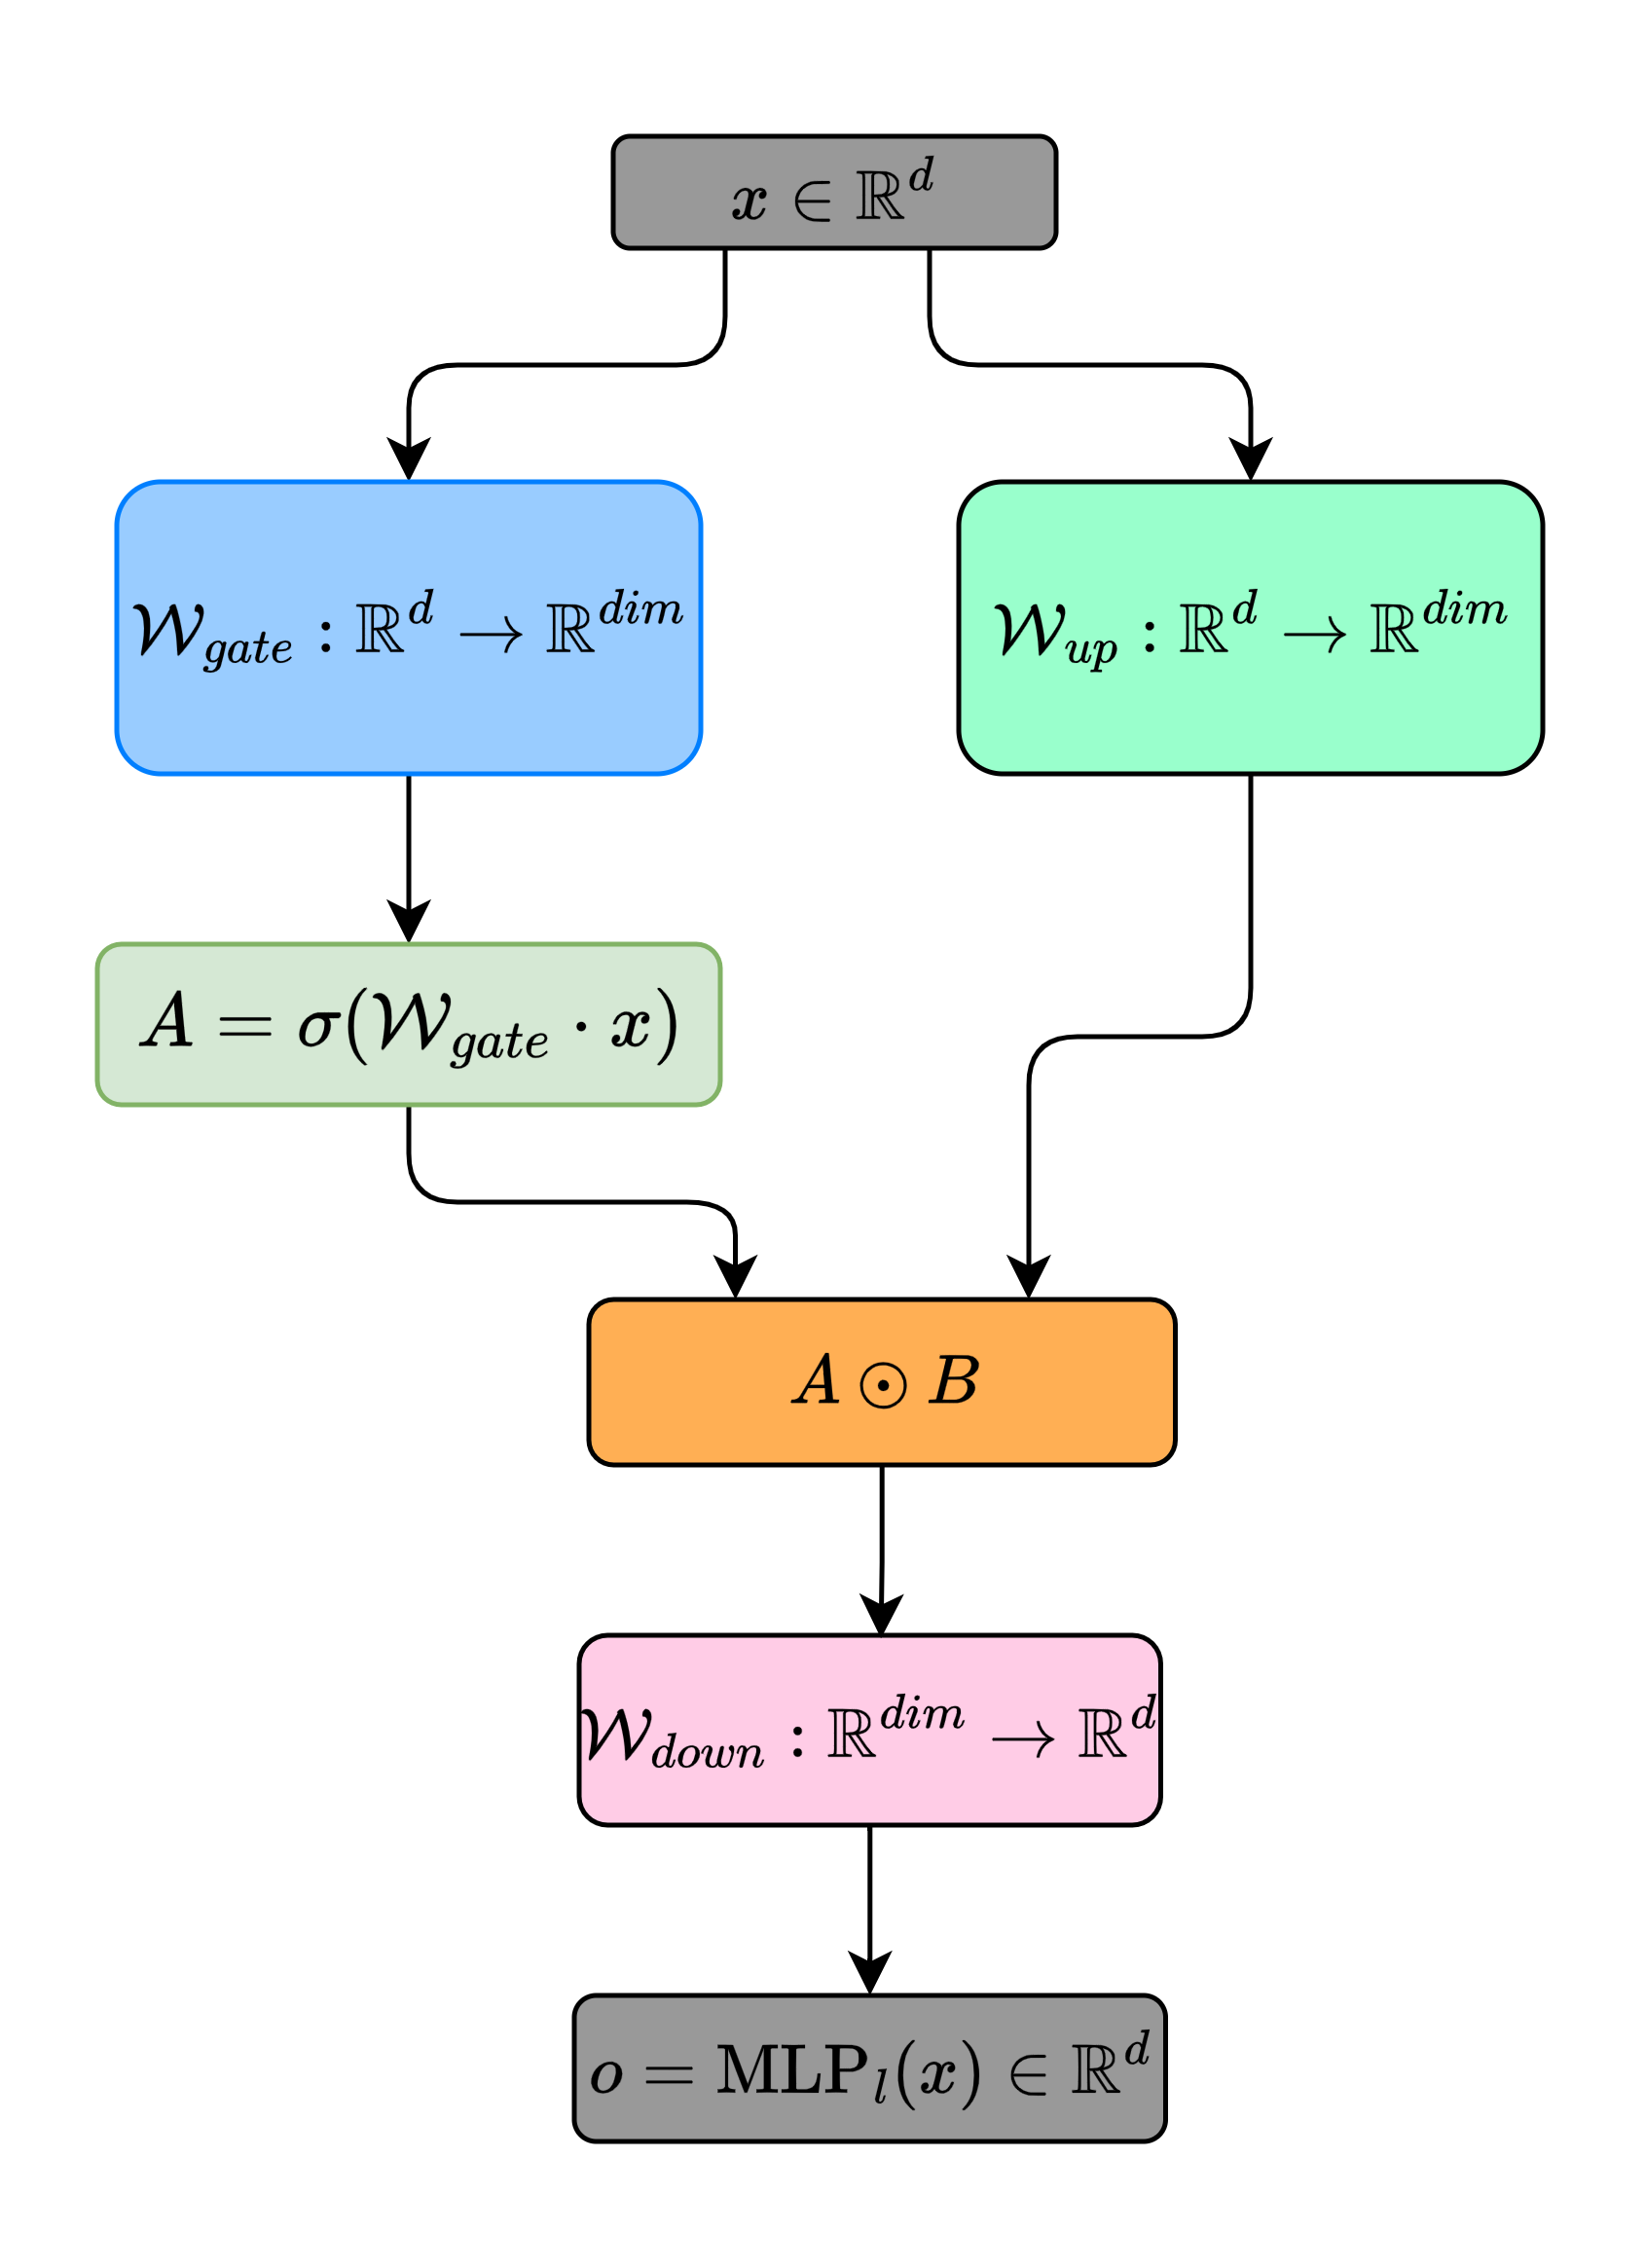
\includegraphics[width=0.65\linewidth]{images/interactive-Page-4.drawio.png}
\caption{SwiGLU MLP architecture in Llama-3-8B. STAMP targets all three weight matrices $\mathcal{W}_{\mathrm{gate}}$, $\mathcal{W}_{\mathrm{up}}$, and $\mathcal{W}_{\mathrm{down}}$ via pseudoinverse updates.}
\label{fig:mlp_architecture}
\end{figure}

\subsection{General Framework}
Figure~\ref{fig:framework} illustrates the end-to-end RePAIR pipeline. During normal operation, $\mathcal{M}_{\textit{patient}}$ processes user prompts to produce responses $r_t = \mathcal{M}_{\textit{patient}}(p_t)$. In parallel, $\mathcal{M}_{\textit{watchdog}}$ monitors the dialogue history $H_t = \{(p_{t-k}, r_{t-k}), \ldots, (p_t, r_t)\}$ over the last $k$ turns and classifies the user's latest message as either \textit{chat} or \textit{unlearn}.

Upon detecting an unlearning request, $\mathcal{M}_{\textit{watchdog}}$ extracts the target pair $(p_f, r_f)$ from $H_t$ and forwards it to $\mathcal{M}_{\textit{surgeon}}$, which generates the repair code $C_t = \mathcal{M}_{\textit{surgeon}}(p_f, r_f)$. The generated code produces the unlearning procedure described in Section~\ref{sec:stamp}, which is \textit{training-free} and operates on a single forget sample $(p_f, r_f)$, transforming $\mathcal{M}_{\textit{patient}}$ into $\mathcal{M}_{\textit{healed}}$. Post-unlearning, $\mathcal{U}$ interacts directly with $\mathcal{M}_{\textit{healed}}$.

\subsection{STAMP: Steering Through Activation Manipulation with Pseudoinverse}
\label{sec:stamp}
We now describe the unlearning method executed by $\mathcal{M}_{\textit{surgeon}}$ on $\mathcal{M}_{\textit{patient}}$. The core idea is to steer forget-set MLP activations toward a refusal distribution via a closed-form weight update, requiring no gradient computation. As illustrated in Figure~\ref{fig:mlp_architecture}, each MLP layer applies three weight matrices:
\begin{equation}
o = W_{\text{down}} \cdot (\sigma(W_{\text{gate}} \cdot x) \odot W_{\text{up}} \cdot x)
\end{equation}
where $x \in \mathbb{R}^d$ is the layer input, $\sigma$ is the SiLU activation, and $\odot$ denotes element-wise multiplication. Since $W_{\text{down}}$ is the only matrix whose output directly determines the MLP output $o$, STAMP applies its closed-form pseudoinverse update to $W_{\text{down}}$, while $W_{\text{gate}}$ and $W_{\text{up}}$ remain frozen; this avoids inverting the SiLU nonlinearity and keeps the update exact rather than approximate.

We target the feed-forward block specifically because factual and world knowledge in transformer LLMs is predominantly stored and recalled through MLP/FFN layers, which act as key-value memories, rather than through attention, which primarily routes information between tokens; steering the FFN output is therefore a more direct lever for suppressing a specific fact than intervening on attention. Moreover, this update rule is architecture-agnostic: STAMP requires only that the targeted matrix satisfy a linear map $o = W \cdot x$ between an observable input and output, and thus applies to the final linear projection of any feed-forward block--not exclusively SwiGLU--including standard ReLU- or GELU-gated MLPs, wherever such a matrix exists.

Given the forget pair $(p_f, r_f)$ extracted by $\mathcal{M}_{\textit{watchdog}}$, we construct the forget set $\mathcal{D}_f = \{(p_f, r_f)\}$ and the retain buffer $\mathcal{D}_r$ (Section~\ref{sec:PS}), along with a reference set $\mathcal{D}_{\textit{ref}}$ of natural refusal prompts. Notably, $\mathcal{D}_f$ can consist of a single sample, where most existing methods fail, whereas STAMP operates effectively at this granularity. 

We extract MLP activations at layer $l$ for all three sets. Since base models such as Llama-3-8B~\cite{grattafiori2024llama} lack explicit refusal training, we exploit their tendency to echo inputs: prompting with ``I don't know'' produces consistent refusal-style activations without additional training. The steering vector, encoding the direction from forget to refusal, is computed as:
\begin{equation}
\mathbf{r}_{\mathrm{\textit{SV}}} = \frac{1}{|\mathcal{D}_{\mathrm{ref}}|} \sum_{x \in \mathcal{D}_{\mathrm{ref}}} \mathrm{MLP}_l(x) - \frac{1}{|\mathcal{D}_f|} \sum_{x \in \mathcal{D}_f} \mathrm{MLP}_l(x) \in \mathbb{R}^{d}
\label{eq:steering_vector}
\end{equation}

Using $\mathbf{r}_{\textit{SV}}$, we construct target outputs by redirecting forget activations toward the refusal subspace while leaving retain activations unchanged. We collect inputs $\mathbf{X} = [x_1; \ldots; x_n] \in \mathbb{R}^{n \times d}$ from $\mathcal{D}_f$, $\mathcal{D}_r$, and $\mathcal{D}_{\textit{ref}}$, and compute desired outputs as follows: if $x \in \mathcal{D}_f$, then $\mathbf{o}'(x) = \mathrm{MLP}_l(x) + \mathbf{r}_{\textit{SV}}$; otherwise, $\mathbf{o}'(x) = \mathrm{MLP}_l(x)$ remains unchanged. The final target matrix $O' \in \mathbb{R}^{n \times d}$ is obtained by stacking all $\mathbf{o}'(x)$.
Let us consider the MLP output for input $\mathbf{X}$:
\begin{equation}
O = \mathbf{X} \cdot W_{\mathrm{old}}
\end{equation}
We seek $W_{\mathrm{new}}$ such that:
\begin{equation}
\mathbf{X} \cdot W_{\mathrm{new}} = O'
\end{equation}
\begin{equation}
W_{\mathrm{new}} = \mathbf{X}^{-1} O'
\end{equation}

\begin{table}[htbp]
\centering
\caption{Memory and computational cost comparison across methods for a single-layer intervention.}
\label{tab:cost_comparison}
\small
\renewcommand{\arraystretch}{1.3}
\begin{tabularx}{\columnwidth}{l|>{\centering\arraybackslash}X>{\centering\arraybackslash}X>{\centering\arraybackslash}X}
\Xhline{1.15pt}
\textbf{Method} & \textbf{Time Complexity} & \textbf{Memory} & \textbf{Training-Free} \\
\Xhline{1.15pt}
Full FT & $\mathcal{O}(E \cdot n \cdot L \cdot d \cdot d_{\mathrm{dim}})$ & $\sim6\times$ model & No \\
\rowcolor{gray!15}
LoRA (all $L$) & $\mathcal{O}(E \cdot n \cdot L \cdot r \cdot d)$ & Model + $2rLd$ & No \\
LoRA (1 layer) & $\mathcal{O}(E \cdot n \cdot r \cdot d)$ & Model + $2rd$ & No \\
\rowcolor{gray!15}
\textbf{STAMP} & $\mathcal{O}(d^3)$ & $d^2$ & Yes \\
\textbf{STAMP-LR} & $\mathcal{O}(r^3 + r^2 \cdot d)$ & $2rd$ & Yes \\
\Xhline{1.15pt}
\end{tabularx}
\end{table}

In Table~\ref{tab:cost_comparison} summarizes the computational and memory trade-offs across methods.

\begin{table*}[htbp]
\centering
\caption{Comparison of STAMP and STAMP-LR with SoTA baselines on Llama-3-8B across three unlearning tasks.}
\label{tab:STAMP-Comparison}
\renewcommand{\arraystretch}{1.05}
{\small
\begin{tabularx}{\textwidth}{l|*{4}{>{\centering\arraybackslash}X}|*{4}{>{\centering\arraybackslash}X}|*{4}{>{\centering\arraybackslash}X}}
\Xhline{1.15pt}
\multirow{2}{*}{\vspace{-0.2cm}\textbf{Method}}  &
\multicolumn{4}{c|}{\textbf{Harmful Knowledge Removal}} &
\multicolumn{4}{c|}{\textbf{Misinformation Removal}} &
\multicolumn{4}{c}{\textbf{Personal Data Erasure}} \\
\cmidrule(lr){2-5}\cmidrule(lr){6-9}\cmidrule(lr){10-13}
& $\mathrm{Acc}_\textit{f}{\downarrow}$ & $\mathrm{Acc}_\textit{r}{\uparrow}$ & Utility$\downarrow$ & RTE 
& $\mathrm{Acc}_\textit{f}{\downarrow}$ & $\mathrm{Acc}_\textit{r}{\uparrow}$ & Utility$\downarrow$ & RTE 
& $F\text{-}RL{\downarrow}$ & $R\text{-}RL{\uparrow}$ & Utility$\downarrow$ & RTE  \\
\Xhline{1.15pt}
Base
  & 75.30 & 78.50 & 5.90 & N/A
  & 83.70 & 86.30 & 5.75 & N/A
  & 0.87  & 0.89  & 5.01 & N/A \\
\rowcolor{gray!15}
Oracle
  & N/A    & 77.37 & 6.10 & N/A
  & N/A    & 85.30 & 5.25 & N/A
  & N/A    & 0.90  & 5.01 & N/A \\
\midrule
GA~\cite{yao2024large}
  & 0.00 & 73.27 & 11.27 & 12.25
  & 0.00 & \colorbox{yellow!40}{83.21} & 10.26 & 6.58
  & 0.13 & 0.81  & 10.17 & 10.41 \\
\rowcolor{gray!15}
NPO~\cite{zhang2024negative}
  & 0.00 & 71.37 &  9.27 & 11.17
  & 0.10 & 80.60 & 11.27 & 6.32
  & 0.27 & 0.83  & 10.00 & 9.48 \\
RMU~\cite{li2024wmdp}
  & 0.00 & \colorbox{green!30}{74.63} &  {7.10} & 12.50
  & 0.27 & 82.17 &  8.10 & 6.00
  & 0.16 & 0.75  & {8.07} & 9.36\\
\rowcolor{gray!15}
FLAT~\cite{wang2024llm}
  & 0.01 & \colorbox{yellow!40}{73.92} &  8.36 & 12.13
  & 1.30 & 80.01 &  \colorbox{yellow!40}{6.29} & 7.12
  & 0.33 & 0.79  &  \colorbox{yellow!40}{7.17} & 11.25\\
WGA~\cite{wang2025rethinking}
  & 2.10 & 70.17 & 11.99 & 11.20
  & 2.47 & 78.30 & 10.90 & {5.45}
  & 0.45 & 0.85  &  9.93 & 9.24\\
\rowcolor{gray!15}
ASU~\cite{zade2026attention}
  & 0.90 & 68.39 &  7.91 & 12.13
  & 0.10 & 79.93 &  7.17 & 6.36
  & {0.07} & \colorbox{yellow!40}{0.87}  &  8.18 & 10.57\\
\midrule\midrule
\textbf{STAMP}
  & 0.00 & 70.13 &  \colorbox{green!30}{6.55} & \colorbox{yellow!40}{7.13}
  & 0.00 & 80.13 &  \colorbox{green!30}{6.02} & \colorbox{yellow!40}{4.25}
  & {0.00}  & 0.79  &  \colorbox{green!30}{6.07} & \colorbox{yellow!40}{6.48} \\
\textbf{STAMP-LR}
  & 0.00 & {73.27} & \colorbox{yellow!40}{7.00} & \colorbox{green!30}{4.25}
  & 0.00 & \colorbox{green!30}{84.47} & {7.39} & \colorbox{green!30}{2.57}
  & {0.00}  & \colorbox{green!30}{0.88} & 8.17 & \colorbox{green!30}{4.01} \\
\Xhline{1.15pt}
\end{tabularx}%
}
\end{table*}

\textbf{STAMP: Pseudoinverse Solution:} To resolve this without additional samples, we use the Moore-Penrose pseudoinverse:
\begin{equation}
\mathbf{X}^{+} = (\mathbf{X}^\top \mathbf{X} + \lambda I)^{-1} \mathbf{X}^\top
\end{equation}
\begin{equation}
W_{\mathrm{new}} = \mathbf{X}^{+} \cdot O'
\end{equation}

The computational bottleneck lies in inverting $(\mathbf{X}^\top \mathbf{X} + \lambda I) \in \mathbb{R}^{d \times d}$, which requires $\mathcal{O}(d^3)$ operations.

\textbf{STAMP-LR: Low-Rank Solution:} To address this, we approximate $\mathbf{X} \approx A B$, where $A \in \mathbb{R}^{n \times r}$ and $B \in \mathbb{R}^{r \times d}$, with $r \ll d$:
\begin{equation}
A^{+} = (A^\top A)^{-1} A^\top, \quad
B^{+} = B^\top (B B^\top)^{-1}
\end{equation}
\begin{equation}
W_{\mathrm{new}} = B^{+} \cdot A^{+} \cdot O'
\end{equation}

This reduces complexity to $\mathcal{O}(r^3 + r^2 \cdot d)$, enabling efficient on-device unlearning.

\subsection{Memory and Computational Analysis}
A forward pass through one MLP layer costs $\mathcal{O}(d \cdot d_{\mathrm{dim}})$, while a backward pass costs approximately $2\times$ that of the forward pass. Full fine-tuning over $n$ samples for $E$ epochs across $L$ layers requires $\mathcal{O}(E \cdot n \cdot L \cdot d \cdot d_{\mathrm{dim}})$ computation and approximately $6\times$ model memory. LoRA reduces this to $\mathcal{O}(E \cdot n \cdot L \cdot r \cdot d)$, but still requires backpropagation.

In contrast, STAMP requires only a single forward pass, with complexity $\mathcal{O}(n \cdot d)$ and no gradient computation. STAMP-LR further reduces both memory and computational cost, making it suitable for on-device deployment.

